% 原文 pp.3–11（印刷 pp.1121–1129）
\section{Lecture 1：对称性破缺}

\begin{keytakeaways}
本讲的主题是「对称性破缺」，而讨论的起点是一个概念上的区分：所谓「理论」是一个二元组 $(X,H)$，即辛流形加能量函数（等价地，Poisson 代数加 Hamilton 量）；所谓「实现」则是这一理论的具体表示——经典情形下是相空间上的一个点或一条轨道，量子情形下是 $*$-代数在一个 Hilbert 空间中的不可约表示。

核心数学工具依次是：辛几何与 Hamilton 流、Poisson 代数、$*$-代数的不可约表示、Schrödinger 算符的谱理论（基态唯一性），以及欧氏路径积分与 Feynman–Kac 公式加小 $\hbar$ 驻相分析。

主要结论有三条。第一，在量子力学中对称性破缺根本不会发生：Stone–von Neumann 定理保证实现唯一，而一维 Schrödinger 算符的基态波函数不变号，故基态唯一，因而自动对称。

第二，在准经典极限 $\hbar\to0$ 中对称性作为「简并」重新出现：两个定域态 $\psi_\pm$ 在微扰论的任何有限阶都无法区分，其能量差与重叠都是 $e^{-S_0/\hbar}$ 级的非微扰效应。

第三，把同一路径积分论证搬到有限体积的量子场论，结论完全相同——两个真空之间的跃迁振幅由瞬子作用量 $S_0=S_*(\infty)$ 指数压低，因此并不存在真正简并的真空。
\end{keytakeaways}

% ===== 原文 p.3 =====
% 原文页首标题：LECTURE 1 / Symmetry Breaking（已并入本节标题）

本学期我们将继续讨论量子场论，但如今主要关心的是动力学（dynamics），而不是微扰论与纯粹形式化的东西。我们要讨论的这些课题，若想严格处理，比上学期所学的那种形式理论要困难得多。我们会尽量把数学陈述讲得尽可能精确，但有时这会很不容易。总的说来，我们将努力对正在发生的事情形成一个直观的图像，并通过考察具体的例子来阐明它。\footnote{本讲笔记由 Pavel Etingof、David Kazhdan 与 David Morrison 整理。}

\subsection{理论与实现}
% 原文 §1.0：Theories and realizations

［本节是解释性的，由本讲义的整理者所写，目的是制造一种虚假的安全感，也就是制造一种没有根据的感觉：以为我们在本讲的其余部分知道自己所谈论的是什么。不幸的是，事实并非如此——至少，如果把「理解」理解成数学家的通常用法的话。］

就本讲以及随后各讲的目的而言，把理论与它的实现区分开来对我们十分重要。因此，让我们解释一下我们所说的「理论」是什么意思，所说的「它的实现」又是什么意思。这个解释并不是一个数学定义（事实上，要给出一个既严格又有用的定义是很困难的），但我们希望它能使我们谈论的内容更清楚一些。

回忆一下，一个经典物理系统 $\Sigma$ 通常是这样描述的：给出 $\Sigma$ 的状态空间 $X$（一个辛流形，可以是无穷维的），以及一个保持辛结构的时间平移单参数群 $g^t$。于是 $g^t$ 产生一个 Hamilton 流，它由 Hamilton 函数 $H$ 定义。（出于物理上的理由，Hamilton 函数应当整体地存在。）$H$ 称为该系统的 Hamilton 量，或能量函数。应当记住，$H$ 只在相差一个（局部）常函数的意义下才有定义。

在大多数例子中，$H$ 有下界。在这种情形下，总可以把 $H$ 归一化，使得 $H$ 在（$X$ 的每个连通分支上）的下确界为零。

在这种情形下，所谓一个理论（theory），我们指的是一个二元组 $(X,H)$，其中 $X$ 是辛流形，$H:X\to\mathbb{R}$ 是能量函数，且只在相差一个（局部）常函数的意义下有定义。所谓这个理论的一个基态（ground state），我们指的是系统 $\Sigma$ 的一个最低能量的平衡态 $x\in X$，即能量泛函 $H$ 在其中达到全局极小的一个状态。

% ===== 原文 p.4 =====
同一个理论可以有不同的基态。例如，若我们有一个直线上的粒子，其势能为 $U(x)=\frac{g}{4!}(x^2-a^2)^2$，那么空间 $X$ 就是以 $(x,p)$ 为坐标的相平面 $\mathbb{R}^2$，Hamilton 量为 $\frac{p^2}{2}+U(x)$，而有两个基态 $(a,0)$ 与 $(-a,0)$。

经常地，一个经典系统 $\Sigma$ 可以由某个 Lagrange 量（Lagrangian）$\mathcal{L}$ 来描述，它定义在时空 $V$ 上某个场空间 $S$ 上。此时它的状态空间就是 $\mathcal{L}$ 的极值场所构成的空间 $X\subset S$。正如我们以前看到过的，空间 $X$ 上带有一个自然的闭二维形式 $\omega$，它是非退化的，因而在 $X$ 上定义一个辛结构。此外，时间平移群作用在 $X$ 上并保持 $\omega$。因此，由这个单参数群在 $X$ 上生成的流是 Hamilton 流，并由一个 Hamilton 函数 $H$ 定义。

然而，应当记住，用一个 Lagrange 量来描述理论并不是内蕴的，因为定义在不同场空间 $S$ 上的不同 Lagrange 量可以定义同一个理论。的确，例如考虑定义在 $S_1=C^\infty(\mathbb{R},M)$ 上的 Lagrange 量 $\mathcal{L}_1=\int x'(t)^2dt/2$，其中 $M$ 是 Riemann 流形。这个 Lagrange 量定义测地流。此时状态空间是 $T^*M$，Hamilton 函数是 $p^2/2$。另一方面，我们可以写下定义在空间 $S_2=C^\infty(\mathbb{R},T^*M)$ 上的 Lagrange 量 $\mathcal{L}_2=\int(x'(t)p(t)-p^2(t)/2)dt$。容易看出，这两个 Lagrange 量定义同一个理论。

% [Tutor Note: 「容易看出」背后是一个恒等式：$\mathcal{L}_2=\int(\dot x\,p-\frac{p^2}{2})dt=\int\frac{\dot x^2}{2}dt-\frac12\int(\dot x-p)^2dt$。也就是说 $\mathcal{L}_2$ 与 $\mathcal{L}_1$ 只相差一个「在壳为零」的平方项：把 $p$ 当作辅助场，其运动方程 $p=\dot x$ 代回即得 $\mathcal{L}_1$。二者给出同一组极值轨道（测地线）、同一辛约化后的相空间 $T^*M$，但场空间不同（$C^\infty(\mathbb{R},M)$ 与 $C^\infty(\mathbb{R},T^*M)$）。这正是「理论不等于 Lagrange 量」的最简单例证：$\mathcal{L}_2$ 就是 $\mathcal{L}_1$ 的一阶（Hamilton 型）形式，两者相差一个全导数加上这个平方项。]

我们将考虑相对论不变的理论 $(X,H)$，即在 $X$ 上有 Poincaré 群 $\mathbf{P}$ 的作用、且该作用保持辛结构的理论（当系统由 Lagrange 量定义时，群 $\mathbf{P}$ 作用在 $S$ 上并保持该 Lagrange 量，因此它作用在 $X$ 上并保持辛结构）。时间平移群是 $\mathbf{P}$ 的子群，所以 $\mathbf{P}$ 也保持能量函数 $H$。在非病态的例子中（事实上，在任何能量函数的极小值确实被取到的例子中），相对论性场论的基态是 $\mathbf{P}$ 不变的。

回忆一下，定义一个辛流形 $X$ 与定义一个 Poisson 代数 $A=C^\infty(X)$ 是同一件事（$X$ 可以从 $A$ 的谱重新构造出来）。因此，我们可以说一个理论是一个二元组 $(A,H)$，其中 $A$ 是 Poisson 代数，$H\in A$。Poisson 代数 $A$ 称为该系统的可观测量代数（algebra of observables）。

现在让我们考虑量子系统。此时理论的定义与经典情形类似。也就是说，我们把一个量子理论（quantum theory）定义为一个二元组 $(A,H)$，其中 $A$ 是一个 $*$-代数（不必交换），$H$ 是 $A$ 中的一个自伴元，且只在相差一个实数加项的意义下有定义。代数 $A$ 称为量子可观测量（算符）代数。元素 $H$ 一如既往称为 Hamilton 量。这里的一切都依赖于一个实的正参数 $\hbar$（Planck 常数）。

所谓量子理论 $(A,H)$ 的一个实现（realization，或解），我们指的是代数 $A$ 在某个 Hilbert 空间 $\mathcal{H}$ 中的一个不可约 $*$-表示，使得算符 $H$ 的谱有下界（表示按保持 $H$ 的同构来分类）。我们总把 $H$ 归一化，使其谱的最低点为零。空间 $\mathcal{H}$ 称为该系统的（在此实现下的）量子状态空间。当然，同一个理论原则上可以有不同的实现，正如同一个代数可以有不同的表示。

% ===== 原文 p.5 =====
正如我们已经提到过的，我们将关心相对论不变的理论，即 $A$ 上有 Poincaré 群作用、从而其中时间平移子群按 $a\mapsto e^{-itH/\hbar}ae^{itH/\hbar}$ 作用的那些理论。当我们谈论这类理论的一个实现时，我们将假定 $\mathbf{P}$ 通过酉算符作用在 $\mathcal{H}$ 上，而其中时间平移群按 $e^{-itH/\hbar}$ 作用。

所谓量子理论 $(A,H)$ 在一个实现 $\mathcal{H}$ 中的一个量子基态（quantum ground state），我们指的是一个向量 $\Omega\in\mathcal{H}$，它是 $H$ 的一个本征态，且其本征值取尽可能小的值。在维数 $\ge2$ 的相对论不变量子场论中，基态称为真空态（vacuum state），它与 $\mathbf{P}$ 不变的向量是同一回事；此时基态的能量（由 $\mathbf{P}$ 不变性）为零。

\textbf{注（Remark）.}
一般说来，一个量子理论的不可约实现可以有许多基态。例如，对于紧流形上 Dirac 算符的理论，基态就是调和旋量（harmonic spinor）；调和旋量构成的空间可以多于一维。然而，可以证明：对于满足 Wightman 公理的两个或更高维的 Minkowski 空间场论，任何实现都恰有一个真空态。在许多 Wightman 公理不成立的情形中，这一点也成立。这就是为什么在量子场论中，「实现」与「真空态」这两个词可以当作同义词使用。

% [Tutor Note: 「任何实现都恰有一个真空态」是 Wightman 框架下的标准定理，作者未给证明：谱条件（能动量四维矢量落在闭前锥内）加上真空的 Poincaré 不变性，可证不变子空间至多一维；不可约性再把「至多一维」提升为「恰为一维」。作者接着说「Wightman 公理失效时也常成立」，指的是只需要 Osterwalder–Schrader 正性与聚类性质，而不需要完整的公理体系。详见 Streater–Wightman, \textit{PCT, Spin and Statistics, and All That}，或 Haag, \textit{Local Quantum Physics}。]

假定我们有一个已经被量子化的经典理论 $(A_0,H_0)$，相应的依赖于 $\hbar$ 的量子理论族为 $(A,H)$（这里所谓依赖于 $\hbar$ 的族，指的是依赖于无量纲参数 $\hbar/S_0$ 的族，其中 $S_0$ 是一个特征作用量标度）。这意味着我们有一个量子化映射——某个线性映射 $A_0\to A$，记作 $a\mapsto\widehat{a}$，使得 $\widehat{H}_0=H$，且
\[
[\widehat{a},\widehat{b}]=i\hbar\widehat{\{a,b\}}+o(\hbar^2),\qquad \hbar\to0.
\]
在这种情形下，我们说一个范数为 1 的状态 $v\in\mathcal{H}$ 定域于经典状态 $x\in X=\operatorname{Spec}A_0$ 附近，如果对任何 $a\in A_0$ 都有 $\langle v,\widehat{a}v\rangle\to a(x)$（当 $\hbar\to0$）。

现在让我们解释经典基态与量子基态这两个概念之间的联系。假定有一个范数为 1 的量子基态 $\Omega$，它定域在经典状态 $x$ 附近。此时 $x$ 是一个经典基态。的确，$H_0(x)=\lim_{\hbar\to0}\langle\Omega,H\Omega\rangle=0$，并且对任何 $F\in A_0$ 有
\[
\{F,H_0\}(x)=\lim_{\hbar\to0}\frac{1}{i\hbar}\langle\Omega,[\widehat{F},H]\Omega\rangle=0,
\]
所以 $x$ 是 $H_0$ 的一个驻点。

\textbf{注（Remark）.}
并非每个量子基态都定域在某个经典基态附近。有时量子真空态是「弥散」的，它在经典基态的集合上（甚至更远处）具有某种密度分布。我们将在本讲以及本学期的其余部分看到这方面的例子。

给定一个量子理论 $(A,H)$，用关联函数（correlation function）来表示它的实现是方便的。也就是说，给定该系统的一个实现 $\mathcal{H}$ 以及一个基态 $\Omega\in\mathcal{H}$，我们可以定义关联函数 $\langle\Omega,L_1\cdots L_n\Omega\rangle$，其中 $L_i\in A$。由于 $A$ 在 $\mathcal{H}$ 中的作用是不可约的，实现 $\mathcal{H}$ 完全可以由这些关联函数重构出来。

\textbf{注（Remark）.}
在维数 $\ge2$ 的物理上有趣的例子中，不可约性条件并不总是满足。一个典型的反例是 $U(1)$ 规范场论：其中电荷算符与所有局部算符对易。但这里为简单起见，我们将假定这个条件满足。

有时一个量子系统可以由一个 Lagrange 量来定义。与经典情形一样，这并不总是可能的；即使可能，方式也不唯一。

% ===== 原文 p.6 =====
然而，这样的表述对于理解系统的行为非常方便。\footnote{而在实践中，我们本学期将要研究的基本上每一个例子，都可以以相当自然的方式从一个 Lagrange 量导出。} 因此，让我们（通过例子）解释如何从一个 Lagrange 量过渡到 Hamilton 量与算符代数。

我们将从量子力学的场合开始，此时时空只是时间轴。考虑单个玻色子的 Lagrange 量：
\[
\mathcal{L}=\int\left[\frac{(\phi')^2}{2}-U(\phi)\right]dt.
\]
那么，按定义，算符代数由算符 $\phi_0$、$\phi_0'$、$H$ 生成，并满足正则对易关系
\[
[\phi_0,\phi_0']=i\hbar,\qquad [H,\phi_0]=-i\hbar\phi_0',\qquad [H,\phi_0']=i\hbar U'(\phi_0).
\]
定义局部算符 $\phi(t)=e^{iHt/\hbar}\phi_0e^{-iHt/\hbar}$，$\phi'(t)=e^{iHt/\hbar}\phi_0'e^{-iHt/\hbar}$。由上述定义可以推出 $d\phi/dt=\phi'$，并且 $\phi$ 满足 Newton 微分方程
\[
\phi''(t)=-U'(\phi(t)).
\]
形如 $F(\phi(t),\phi'(t))$ 的算符（其中 $F$ 是多项式）称为 $t$ 时刻的局部算符（local operator）（我们这样排列乘积，使得 $\phi'$ 位于 $\phi$ 的右侧）。

算符代数（在拓扑意义下）由算符 $\phi(t_1)\cdots\phi(t_n)$ 张成。因此，理论的一个实现由指定这些算符的期望值——即关联函数——来确定。

在理论的任何实现中，Hamilton 量都由下面的显式公式给出：
\[
H=\frac12(\phi')^2+U(\phi)+C.
\]
的确，差 $H-\frac12(\phi')^2+U(\phi)$ 与 $\phi$ 及 $\phi'$ 对易，故由不可约性它作用为标量。

% [Tutor Note: 上句原文把差写成 $H-\frac12(\phi')^2+U(\phi)$，这是笔误。按字面计算：$[H-\frac12\phi'^2+U(\phi),\phi]=0$，但 $[H-\frac12\phi'^2+U(\phi),\phi']=[H,\phi']+[U(\phi),\phi']=i\hbar U'+i\hbar U'=2i\hbar U'\neq0$，并不与 $\phi'$ 对易。只有 $H-\frac12(\phi')^2-U(\phi)=C$ 才同时与 $\phi,\phi'$ 对易。原文逗号后的正是这个意思（$C$ 为标量），中间那个 $+U(\phi)$ 应读作 $-U(\phi)$。]

% [Tutor Note: 三条正则对易关系并不互相独立。若已取 $\phi_0'$ 为动量、$H=\frac12\phi_0'^2+U(\phi_0)+C$，则由 $[f(q),p]=i\hbar f'(q)$ 可直接得到 $[H,\phi_0]=-i\hbar\phi_0'$ 与 $[H,\phi_0']=i\hbar U'(\phi_0)$；真正作为量子化输入的是第一条加上「$H$ 是 $\phi_0'$ 的二次型」这一形式。符号上易错之处：Heisenberg 方程是 $\dot\phi=\frac{i}{\hbar}[H,\phi]$，代入 $[H,\phi_0]=-i\hbar\phi_0'$ 才得到 $\dot\phi=\phi'$；若把 $[\phi_0,\phi_0']$ 写成 $-i\hbar$，$\dot\phi$ 会整体变号，Newton 方程也随之反号。此外「$\phi'$ 置于 $\phi$ 右侧」的排序约定在本例中无关紧要（$U=U(\phi)$），但当 $F$ 含 $\phi'$ 的高次项时会改变算符乘积的定义。]

现在考虑量子场论。我们首先考虑时空为 $V=L\times\mathbb{R}$ 的理论，其中 $L$ 是一个格点（有限或无限）。设 $\nabla_L$ 为格点上的离散梯度算符。考虑 Lagrange 量
\[
\mathcal{L}=\sum_{x\in L}\int dt\left[\frac12\left(\phi_t^2(x,t)-(\nabla_L\phi(x,t))^2\right)-U(\phi(x,t))\right].
\]
此时算符代数由算符 $\phi(x,0)$、$\phi_t(x,0)$（$x\in L$）以及 $H$ 生成，满足对易关系
\[
\begin{aligned}
&[\phi(x,0),\phi_t(x,0)]=i\hbar,\qquad [H,\phi(x,0)]=-i\hbar\phi_t(x,0),\\
&[H,\phi_t(x,0)]=i\hbar\left[-\Delta_L\phi(x,0)+U'(\phi(x,0))\right],
\end{aligned}
\]
（其中 $\Delta_L$ 是格点 Laplacian），并且当 $x\neq y$ 时 $\phi(x,0),\phi'(x,0)$ 与 $\phi(y,0),\phi'(y,0)$ 对易（因果性）。局部算符 $\phi(x,t),\phi'(x,t)$ 按上面同样的方式定义。（注意：由于 $H$ 不与 $\phi$ 对易，当 $t_1\neq t_2$ 时算符 $\phi(x_1,t_1)$ 与 $\phi(x_2,t_2)$ 一般并不对易。）

% ===== 原文 p.7 =====
与前面一样，算符代数由算符 $\phi(x_1,t_1)\cdots\phi(x_n,t_n)$ 张成。因此，理论的一个实现由这些算符的期望值——关联函数——所确定。

与量子力学的情形一样，在任何实现中我们都可以显式地算出 Hamilton 量。也就是说，Hamilton 量具有形式 $H=\sum_{x\in L}H_x$，其中
\[
H_x=\frac12\left(\phi_t^2(x,0)+(\nabla_L\phi(x,0))^2\right)+U(\phi(x,0))+C_x.
\]

\textbf{注（Remark）.}
当然，如果格点 $L$ 是无限的，$H$ 的定义可能有问题，因为对 $L$ 的求和可能发散。然而，由于 $H$ 与其他算符的对易子有良好定义，人们可以希望常数 $C_x$ 实际上能被调整得使该和收敛。在许多情形下这确实成立。

% [Tutor Note: $C_x$ 的可调性等价于对每个格点作正规序（normal ordering）：物理上只有 $H$ 的对易子进入运动方程，而常数在对易子中抵消，故 $C_x$ 可任取。在无限格点上 $\sum_x C_x$ 按体积发散，但只要逐点取 $C_x$ 使 $\langle\Omega|H_x|\Omega\rangle=0$，$H$ 的矩阵元就是有限的。连续极限下这一自由度变成真空能（宇宙学常数）的不确定性，只能由引力或额外的对称性要求来固定。]

现在让我们考虑连续时空中的场论。此时算符代数与 Hamilton 量的定义，与上面考虑过的离散空间情形类似。也就是说，算符代数将由算符 $\phi(x,0)$、$\phi_t(x,0)$，以及 $H_b$（$b\in\mathfrak{p}$）生成，其中 $\mathfrak{p}$ 是 Poincaré 群 $\mathbf{P}$ 的 Lie 代数，而 $\phi,\phi_t$ 与 $H_b$ 之间的对易关系与上面类似。

然而，我们将面临一个额外的问题——现在像 $\phi^2(x,t)$ 这样的表达式可能没有良好定义，因为存在紫外发散（ultraviolet divergence）。如果我们出发时的 Lagrange 量是可重整化的，这个问题可以用上学期讨论过的紫外重整化理论来治愈。在此情形下，局部算符的代数并不完全是一个代数，而是一个 OPE 代数（即带有算符乘积展开的代数）。几乎从来不可能精确算出这个代数的结构常数（二维的有理共形场论是主要的例外），但可以在微扰展开中把它算到任何有限阶。一般说来，对于连续空间，与离散空间的情形相比我们还有额外的分析上的困难，但这些困难在本讲中并不很重要，所以我们不在这里讨论它们。我们只需要一个粗略的总体图像，这已在本导引中勾画出来了。

\subsection{什么是对称性破缺，以及它为何不在量子力学中发生}
% 原文 §1.1：What is symmetry breaking, and why it does not happen in quantum mechanics

假定我们有某个经典物理理论 $(A,H)$，它具有对称群 $G$。让我们问下面这个问题：这个理论是否有 $G$ 不变的基态？

如果我们有一个量子理论 $(A,H)$，它具有对称群 $G$，那么在实现与真空态之间没有区别的情形下，这个问题的正确类比是：这个理论是否有 $G$ 不变的实现？

如果答案是否定的，人们就说对称性破缺（broken）；如果答案是肯定的，就说对称性保持（preserved）。

在经典力学与经典场论中，对称性破缺很容易发生。例如，考虑直线上一个质量为 1 的经典粒子，其势能为 $U(x)=g(x^2-a^2)^2/4!$，其中 $a>0$、$g>0$。这个粒子的状态空间是以 $x,p$ 为坐标的平面，其 Hamilton 量为 $\frac{p^2}{2}+U(x)$。群 $G=\mathbb{Z}/2\mathbb{Z}$ 通过 $(x,p)\to(-x,-p)$ 作用在状态空间上，该作用保持运动方程，而存在两个

% ===== 原文 p.8 =====
最低能量态：$s_+=(a,0)$、$s_-=(-a,0)$，它们被 $G$ 互换。但不存在 $G$ 不变的最低能量态。

在量子力学中，对称性破缺不会发生。让我们对玻色子的理论证明这一点：其算符代数由算符 $x_i,p_i$（$i=1,\dots,n$）生成，满足 Heisenberg 代数关系，而 Hamilton 量为 $H=\frac{p^2}{2}+U(x)$。该理论在 $\mathcal{H}=L^2(\mathbb{R}^n)$ 中有一个实现，其中 $x_i$ 通过乘以坐标函数作用，$p_i=-i\hbar\frac{\partial}{\partial x_i}$。众所周知，这个表示是不可约的。势 $U$ 的任何对称群 $G$ 也（射影地）作用在 $\mathcal{H}$ 上。因此，对称性破缺不会发生。

\textbf{注（Remark）.}
事实上，按 Stone–von Neumann 定理，$\mathcal{H}$ 是这个理论的唯一实现。

对于具有实 Lagrange 量的玻色子，我们实际上可以给出更强的论断。也就是说，不仅实现是唯一的，而且基态也是唯一的（从而在任何 $U$ 的对称群下不变）。为简单起见，我们只对直线上单个玻色子的情形证明这一点，但我们给出的论证可以推广到任意维空间中的任意多个玻色子。

我们将考虑直线上的单个玻色子，处于如上所述的势 $U(x)$ 的场中。

\textbf{定理 1.1.}
设 $H=-\frac12\frac{d^2}{dx^2}+U(x)$ 是任一 Schrödinger 算符，使得势 $U(x)$ 在无穷远处趋于 $+\infty$（从而 $H$ 具有离散谱）。设 $E_0$ 是 $H$ 的最小本征值。则存在唯一的（相差一个因子）函数 $\psi\in L^2(\mathbb{R})$（称为基态波函数），使得 $H\psi=E_0\psi$。

\textbf{证明.}
对任何 $f\in L^2(\mathbb{R})$ 我们有
\begin{equation}
  \tag{1.1}
  \label{eq:1-1}
  (f,Hf)=\int_{-\infty}^{\infty}\left(\frac12|f'(x)|^2+U(x)|f(x)|^2\right)dx.
\end{equation}
因此，$\psi$ 由如下条件刻画：它是能量泛函 $E(f):=(f,Hf)$ 在球面 $\|f\|=1$ 上的全局极小点。$\psi$ 的唯一性的证明依赖于下面的引理。

\textbf{引理.}
若 $\psi$ 是 (1.1) 的一个实全局极小点，则 $\psi$ 具有不变的符号。

\textbf{引理的证明.}
设 $E(\psi)=E_0$。假定 $\psi$ 在点 $x_0$ 处变号。由于 $\psi$ 满足 Euler–Lagrange（$=$Schrödinger）方程 $H\psi=E_0\psi$，我们有 $\psi'(x_0)\neq0$。考虑函数 $|\psi|$。显然 $E(|\psi|)=E(\psi)=E_0$，但 $|\psi|$ 不光滑，故它不满足 Euler–Lagrange 方程 $Hf=E_0f$，因而不能是 $E$ 的全局极小。于是 $E$ 在球面上的最小值小于 $E_0$——矛盾。

现在容易证明该定理。如果 $H\psi=E_0\psi$ 的解空间多于一维，则存在两个线性无关、彼此正交的实解 $\psi_1,\psi_2$。另一方面，它们都必须具有不变的符号，所以 $(\psi_1,\psi_2)\neq0$——矛盾。$\square$

% [Tutor Note: 引理的证明有两处跳步，都值得补上。(a)「$\psi$ 在 $x_0$ 变号 $\Rightarrow\psi'(x_0)\neq0$」依赖 $H\psi=E_0\psi$ 是二阶线性 ODE：若 $\psi(x_0)=\psi'(x_0)=0$，由解的唯一性得 $\psi\equiv0$，与 $\|\psi\|=1$ 矛盾。(b)「$E(|\psi|)=E(\psi)$」需要 $|\psi|\in H^1$ 且链式法则在 $H^1$ 中几乎处处成立（Stampacchia 引理）；而「$|\psi|$ 不光滑故不是驻点」用到椭圆正则性：$U$ 光滑时 $H\psi=E_0\psi$ 的弱解实解析，而 $|\psi|$ 在 $x_0$ 处有尖角，故不可能是解。这里的「基态非简并」本质上是一维的 Sturm 振荡定理（或 Perron–Frobenius 正性）；在 $d\ge2$ 维对一般 $U$ 并不成立，只能对谱的下端成立。]

考虑量子理论中并不存在的对称性破缺如何在准经典极限中出现，是有益的。为此，我们应当引入 Planck 常数 $\hbar$，并考虑依赖于 $\hbar$ 的 Hamilton 量
\begin{equation}
  \tag{1.2}
  \label{eq:1-2}
  H=-\frac{\hbar^2}{2}\frac{d^2}{dx^2}+U(x),
\end{equation}

% ===== 原文 p.9 =====
其中 $U(x)=g(x^2-a^2)^2/4!$。设 $E_0,E_1$ 分别是 $H$ 在偶函数空间与奇函数空间中的最小本征值，$\psi_0,\psi_1$ 为相应的本征向量。我们假定 $\psi_0,\psi_1$ 具有单位范数，并如此归一化，使得 $\psi_0(0)>0$、$\psi_1'(0)>0$。用与上面相同的方式容易证明，$\psi_1$ 在区域 $x>0$ 与 $x<0$ 中都不变号。定义
\[
\psi_+=\frac{1}{\sqrt2}(\psi_0+\psi_1),\qquad \psi_-=\frac{1}{\sqrt2}(\psi_0-\psi_1).
\]

于是可以证明下面的结论。

\textbf{定理 1.2.}
(i) 当 $\hbar\to0$ 时，$E_0,E_1\sim a\hbar\sqrt{g/4!}$，且 $E_1-E_0\sim Ce^{-S_0/\hbar}$，其中 $S_0$ 是一个正常数。

(ii) 在分布的意义下，
\begin{equation}
  \tag{1.3}
  \label{eq:1-3}
  \lim_{\hbar\to0}|\psi_\pm|^2=\delta(x\mp a).
\end{equation}

这个定理表明，对于非常小的 $\hbar$，虽然只有一个能量为 $E_0$ 的最低能量态 $\psi_0$，但还存在另一个定态 $\psi_1$，其能量 $E_1$ 与最低能量几乎不可区分；而在 $\psi_0,\psi_1$ 张成的二维空间中，有两个彼此正交的态 $\psi_+,\psi_-$，分别定域在经典平衡态 $a,-a$ 附近。态 $\psi_+,\psi_-$ 不是定态（即不是 $H$ 的本征向量），但它们「不是定态」这一点在 $\hbar$ 的任何有限阶上都是不可区分的（事实上，$H\psi_\pm$ 与 $\psi_\pm$ 之间的夹角被 $\mathrm{const}\cdot e^{-S_0/\hbar}$ 所控制）。特别地，量子理论中的对称性恢复在微扰论层面上是看不到的。

这样，我们就看到了对称性如何在准经典极限中丢失。人们可以从稍微不同的角度来考察这一效应，即考察对称性在量子化过程中如何出现。

回忆一下，我们有两个经典最低能量态 $a,-a$，在它们附近算符 $H$ 近似看起来像一个谐振子。因此，我们可以按微扰的方式寻找 $H$ 的本征函数，其形式为
\begin{equation}
  \tag{1.4}
  \label{eq:1-4}
  \begin{aligned}
    \widetilde{\psi}_\pm(x)&=f_\pm\left(\frac{x\mp a}{\sqrt{\hbar}}\right),\\
    f_\pm(z)&=(\pi\hbar)^{-1/4}g^{1/8}e^{-\sqrt{g}\,z^2/2}
      \left(1+u_1(z)\hbar^{1/2}+u_2(z)\hbar+\dots\right).
  \end{aligned}
\end{equation}
（这个展开的第 0 项就是谐振子的最低本征函数。）容易看出，形如 (1.4) 的实「本征函数」在归一化为单位范数后，对每个符号都是唯一的。

% [Tutor Note: (1.4) 与定理 1.2(i) 在数值上并不自洽，值得动手核一遍。由 $U=\frac{g}{4!}(x^2-a^2)^2$ 得 $U''(\pm a)=\frac{ga^2}{3}$，故谐振子频率与最低能级应为 $\omega=\sqrt{U''(\pm a)}=a\sqrt{g/3}$、$E_0\sim\frac{\hbar\omega}{2}=a\hbar\sqrt{g/12}$；而定理 1.2(i) 写的是 $a\hbar\sqrt{g/4!}=a\hbar\sqrt{g/24}$，比它小一个因子 $\sqrt2$。再看 (1.4)：指数 $e^{-\sqrt g z^2/2}$ 与预因子 $(\pi\hbar)^{-1/4}g^{1/8}$ 恰好是取 $\omega=\sqrt g$ 的谐振子基态（此时 $\int|f_\pm|^2dz=1$，乘以 $dx=\sqrt\hbar\,dz$ 后范数为 1），而不是取 $\omega=a\sqrt{g/3}$。三处相差的都是 $O(1)$ 因子，不影响「$E_0\sim\frac12\hbar\omega$、能级劈裂 $\propto e^{-S_0/\hbar}$」这些定性结论；但若要作定量估计，应以 $\omega=\sqrt{U''(\pm a)}$ 为准。]

现在可以看到以下几点。

(i) 形式级数 $f_\pm(z)$ 并不收敛。然而，它们表示实际函数 $\psi_\pm(z\sqrt{\hbar}\pm a)$（其中 $\psi_\pm$ 如上）的渐近展开，这些实际函数在 $[0,\infty)$ 上关于 $\hbar$ 从右侧光滑，但不是解析的。

(ii) 形式级数 $\widetilde{\psi}_\pm(x)$ 是 $H$ 的具有相同本征值的本征函数。另一方面，实际函数 $\psi_\pm(x)$ 并不是 $H$ 的本征向量，尽管它们「不是本征向量」的程度是指数小的。$H$ 的实际最低本征向量在相差一个因子的意义下唯一，且等于 $\psi_0=\frac{1}{\sqrt2}(\psi_++\psi_-)$。特别地，它是 $G$ 不变的，而 $\psi_+,\psi_-$ 不是。

(iii) 设 $W^n_+(t_1,\dots,t_n)$、$W^n_-(t_1,\dots,t_n)$ 是用形式真空 $\widetilde{\psi}_+,\widetilde{\psi}_-$ 微扰地（用 Feynman 演算）算出的关联函数。则 $W^n_+,W^n_-$

% ===== 原文 p.10 =====
不能作为我们量子理论任何实现的关联函数的小 $\hbar$ 渐近展开。然而，平均值 $\frac12(W^n_++W^n_-)$ 确实能作为这样的渐近展开。

这说明，当人们从微扰的框架走到非微扰的框架时，对称性在量子化中是如何出现的。

\subsection{有限体积的量子场论中依然没有对称性破缺}
% 原文 §1.2：Still no symmetry breaking in quantum field theory in finite volume

在转到量子场论之前，我们再给出一个论证（在物理的严格性水平上），说明为什么量子力学中没有对称性破缺（这个论证与其说是证明，不如说是解释）。它基于路径积分方法。它既不用 Heisenberg 代数的表示论，也不用基态波函数的正性，并且有一个优点：它同样适用于「空间」部分为有限体积的时空上的量子场论。

与前面一样，我们将考虑 $\mathbb{Z}/2\mathbb{Z}$ 对称的四次势 $U(x)$。假定对称性破缺真的发生了。那么两个微扰真空 $\widetilde{\psi}_+,\widetilde{\psi}_-$ 确实非微扰地存在，即它们分别作为 Hamilton 量的实际最低本征态 $\psi_+,\psi_-$ 的渐近展开，出现在理论的两个不同实现 $\mathcal{H}_+,\mathcal{H}_-$ 中。考虑空间 $\mathcal{H}=\mathcal{H}_+\oplus\mathcal{H}_-$。向量 $\psi_+,\psi_-\in\mathcal{H}$ 分别「定域」在 $a,-a$ 附近，并且彼此正交。因此，内积 $(\psi_+,e^{-Ht/\hbar}\psi_-)$ 必须为零。现在让我们用路径积分来计算同一个内积。

回忆 Feynman–Kac 公式：
\begin{equation}
  \tag{1.5}
  \label{eq:1-5}
  (\delta_{x_1},e^{-Ht/\hbar}\delta_{x_2})
  =\int_{\phi:[0,t]\to\mathbb{R},\ \phi(0)=x_1,\ \phi(t)=x_2} e^{-S(\phi)/\hbar}\,D\phi,
\end{equation}
其中
\begin{equation}
  \tag{1.6}
  \label{eq:1-6}
  S(\phi)=\int_0^t\left[\frac12(\phi')^2+U(\phi)\right]ds.
\end{equation}

态 $\psi_+,\psi_-$「定域」在 $a,-a$ 附近（也就是说，在适当的归一化之后，它们接近 $a,-a$ 处的 delta 函数）。所以，如果我们相信这种情形下的 Feynman–Kac 公式，就可以用 $\delta(x-a)$、$\delta(x+a)$ 代替它们，并应用 Feynman–Kac 公式。对 (1.5) 的右端使用小 $\hbar$ 的驻相估计，我们将得到
\begin{equation}
  \tag{1.7}
  \label{eq:1-7}
  (\psi_+,e^{-tH/\hbar}\psi_-)\sim Ce^{-S_*(t)/\hbar},
\end{equation}
其中 $S_*(t)$ 是满足 $\phi(0)=-a$、$\phi(t)=a$ 的路径 $\phi:[0,t]\to\mathbb{R}$ 的最小可能作用量。

对于大的 $t$，最小作用量 $S_*(t)$ 在经典轨道 $\phi=\phi_*(\tau)$ 上达到，它是 Euler–Lagrange 微分方程的解，即 Newton 方程
\[
\phi''=\frac{g}{6}\phi(\phi^2-a^2)
\]
满足边界条件 $\phi(0)=-a$、$\phi(t)=a$ 的解。（这样的解存在且唯一。）

% [Tutor Note: 由 (1.5) 到 (1.7) 有三处被压缩的步骤。第一，把 $\psi_\pm$ 换成 $\delta(x\mp a)$ 只是首阶近似：$\psi_\pm$ 的宽度是 $O(\hbar^{1/2})$，由此产生的相对误差为 $O(\hbar)$，这正是 (1.7) 只能写成 $\sim$ 的原因。第二，驻相展开的首项带预因子（单圈行列式，即 Van Vleck–Morette 行列式），这就是 (1.7) 中的 $C$；$C$ 与 $\hbar$ 无关，但对 $t$ 有幂次依赖。第三，$S_*(\infty)$ 可以显式算出：对 $t\to\infty$ 的极限轨道，两端速度趋于零而 $U(\pm a)=0$，故守恒量 $\frac12\dot\phi^2-U(\phi)$ 为零，于是 $\dot\phi=\sqrt{2U}$、$S_*(\infty)=\int_{-a}^{a}\sqrt{2U(\phi)}\,d\phi$；代入 $U=\frac{g}{24}(\phi^2-a^2)^2$ 即得 $S_0=\frac{4a^3}{3}\sqrt{g/12}$。这也解释了为什么 $S_0$ 是「作用量」量纲且与 $\hbar$ 无关。]

% ===== 原文 p.11 =====
\begin{figure}[htbp]
  \centering
  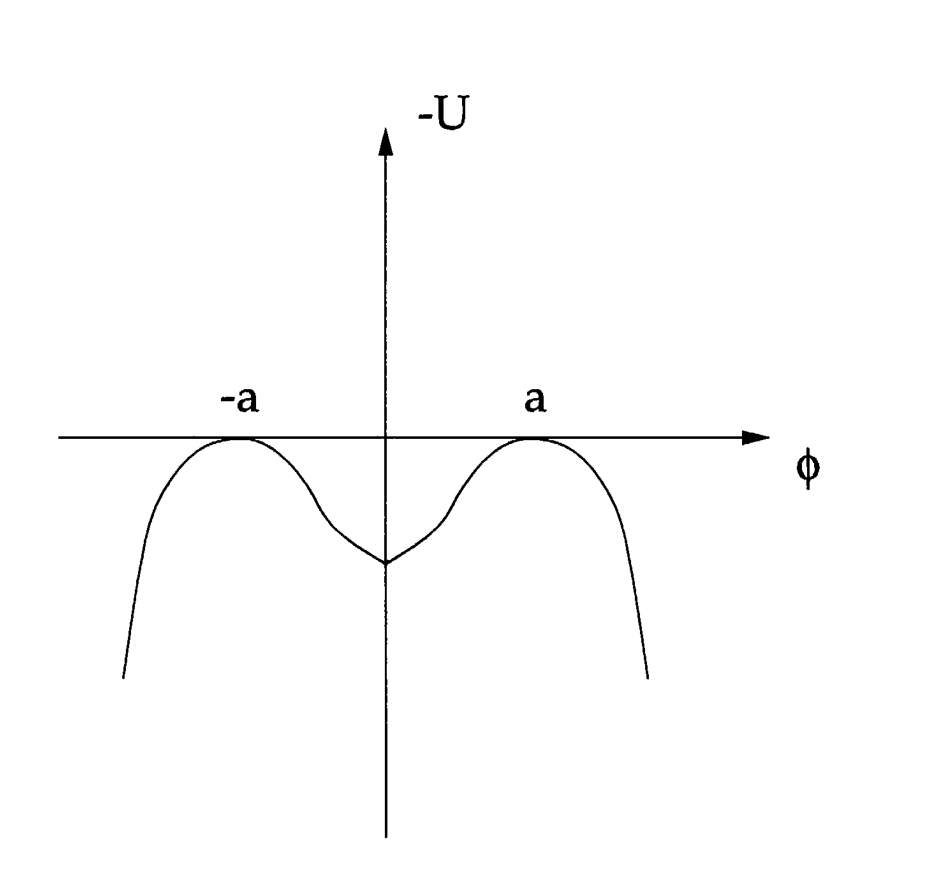
\includegraphics[width=0.5\textwidth]{figs/fig_p011_1.png}
  \caption{「驼峰」形状的势 $-U(x)$：横轴为场 $\phi$，纵轴为 $-U$，两个峰顶位于 $\phi=-a$ 与 $\phi=a$（图中标注 $-a$、$a$），谷底在 $\phi=0$。欧氏路径积分的瞬子解即小球在此势中从一个峰顶滚到另一个峰顶的轨迹。（原文 Figure 1，p.11；原书此图未编号）}
  \label{fig:p11-1}
\end{figure}

\textbf{注 1（Remark 1）.}
函数 $x=\phi_*(\tau)$ 描述一个球在势为 $-U(x)$ 的势场中（如图，形状像驼峰）从一个峰运动到另一个峰。球的初速度取得使从一个峰顶到另一个峰顶所需的时间恰为 $t$。这里把势 $U(x)$ 换成 $-U(x)$ 的理由是：我们做的是欧氏路径积分，也就是说我们做了 Wick 转动 $t\to it$。这个转动把势 $U$ 的 Newton 方程变成势 $-U$ 的 Newton 方程。

\textbf{注 2（Remark 2）.}
当 $t\to\infty$ 时，解 $\phi^*(\tau)$ 有极限；这个极限解在时间平移下唯一。当 $t\to\infty$ 时，解 $\phi^*(\tau)$ 的初速度趋于零。由于在研究 Hamilton 量的低能态时人们关心的是大的 $t$，通常用这个极限解来表达分析，它被称为瞬子（instanton）。

% [Tutor Note: 记号在此处不一致：第 10 页与注 1 用下标星号 $\phi_*(\tau)$、$S_*(t)$，注 2 却写成上标星号 $\phi^*(\tau)$，而下面一句又回到 $S_0=S_*(\infty)$。按上下文二者指同一个极限轨道，译文照原样保留；排版或引用时建议统一为 $\phi_*$，以免与复共轭或「对偶」的常见用法混淆。]

公式 (1.7) 与 $(\psi_+,e^{-Ht/\hbar}\psi_-)$ 为零这一事实矛盾。所以，我们关于存在两个真空的假定是错误的。

\textbf{注（Remark）.}
公式 (1.7) 实际上给出了内积 $(\psi_+,e^{-tH}\psi_-)$ 的正确估计。特别地，$S_0=S_*(\infty)$。这个估计可以用严格的方法加以确认。

在这个论证中，我们从未用到 $\psi_+,\psi_-$ 是实直线上的函数这一事实。我们所使用的只是：它们「定域」在经典平衡态 $a,-a$ 附近，也就是说，对任何局部可观测量 $A$，$A$ 在 $\psi_\pm$ 上的期望值接近相应的经典可观测量在相空间点 $(\pm a,0)$ 处的值。因此，我们的论证与状态空间实现为 $L^2(\mathbb{R})$ 这一选择无关。这使得把这个论证推广到场论的情形变得容易。

考虑时空 $M\times\mathbb{R}$，其中 $M$ 是「空间」。我们将假定已经做了 Wick 转动，使得时空上的度量为 Riemann 乘积度量。我们将假定 $M$ 的体积有限且等于 $V$。

考虑 $M\times\mathbb{R}$ 上带一个标量玻色场 $\phi$ 的场论，它由欧氏 Lagrange 量描述
\begin{equation}
  \tag{1.8}
  \label{eq:1-8}
  \mathcal{L}=\int\left(\frac12(\nabla\phi)^2+U(\phi)\right)dx,
\end{equation}
